\documentclass{article}
\usepackage[utf8]{inputenc}

\title{Neural Networks: Introduction and Overview}
\author{ Nikhil Sardana }
\date{October 2017}

\usepackage{natbib}
\usepackage{graphicx}
\usepackage{mathtools}          %loads amsmath as well
\usepackage{tikz}
\usepackage{pgfplots}

\DeclarePairedDelimiter\Floor\lfloor\rfloor
\DeclarePairedDelimiter\Ceil\lceil\rceil
\begin{document}

\maketitle

\section{Introduction}

Neural networks are fundamental to modern machine learning. In order to understand Convolutional Neural Networks (CNNs), Recurrent Neural Networks (RNNs), Generative Adversarial Networks (GANs), not only is it essential to understand the theory behind standard Neural Networks, but also the mathematics. To ensure complete understand, we only use numpy to build our network, removing any reliance on a library.

\section{The Perceptron}
\begin{center}
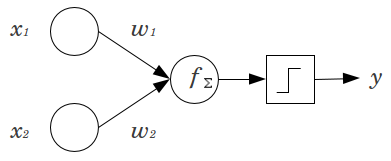
\includegraphics[scale=0.5]{2MVdW}
\end{center}
\subsection{Definition}

A perceptron is the fundamental unit of a Neural Network (which is even called a Multi-Layer Perceptron for this reason). Refer to the diagram above. Perceptrons contain two or more inputs, a weight for each input, a bias, an activation function (the step function) and an output.
For the perceptron above with $2$ inputs, the intermediate value $f(x)$ is as follows
\[f(x) = w_1x_1 + w_2x_2 + b\]
The final output $y$ is just the step function:
\[
  y =
  \begin{cases}
                                   0 & \text{if $f(x) < 0$} \\
  1 & \text{if $f(x) > 0$}
  \end{cases}
\]
\subsection{Visualization}

The purpose of a perceptron is to classify data. Consider the function AND.
\begin{center}
\begin{tabular}{ |c|c|c| } 
 \hline
 x1 & x2 & out \\
 \hline
 0 & 0 & 0 \\ 
 0 & 1 & 0 \\ 
 1 & 0 & 0 \\ 
 1 & 1 & 1 \\ 
 \hline
\end{tabular}
\end{center}
Let's graph this data.
\begin{center}
\begin{tikzpicture}
\begin{axis}[
    axis lines=middle,
    xmin=-1, xmax=2,
    ymin=-1, ymax=2,
    xtick=\empty, ytick=\empty
]
\addplot [only marks] table {
0 0
0 1
1 0
};
\addplot [only marks, mark=o] table {
1 1
};
\addplot [domain=-10:10, samples=2, dashed] {-1*x+1.5};
\end{axis}
\end{tikzpicture}
\end{center}

The line $y = -x + 1.5$ splits this data the best.
Let's rearrange this to get $x + y - 1.5 = 0$. 
Going back to the perceptron formula
\[f(x) = w_1x_1 + w_2x_2 + b\]
we can see that for the optimal perceptron,  $w_1$ and $w_2$ are the coefficients of $x$ and $y$, and $b=-1.5$. If $f(x) > 0$, then $x + y - 1.5>0$. We can see through this example that perceptrons are nothing more than linear functions. Above a line, perceptrons classify data points $1$, below the line, they are $0$.

\subsection{Learning}

How do perceptrons "learn" the best possible linear function to split the data? Perceptrons adjust the weights and bias to iteratively approach a solution.

Let's consider this data:
\begin{center}
\begin{tikzpicture}
\begin{axis}[
    axis lines=middle,
    xmin=-3, xmax=3,
    ymin=-3, ymax=3,
    xtick=1, ytick=1,
]
\addplot [only marks] table {
0 0
-1 2 
1 -2
-1 -2
-2 0
};
\addplot [only marks, mark=o] table {
1 1
0 2
2 2
1 3
1 0
};
\addplot [domain=-10:10, samples=2, dashed] {-1*x+1.5};
\end{axis}
\end{tikzpicture}
\end{center}

The perceptron that represents the dashed line $y+x-1.5=0$ has two inputs, $x_1, x_2,$ with corresponding weights $w_1=1, w_2=1$, and bias $b = -1.5$. Let $y$ represent the output of this perceptron. In the data above, the point $(1, 0)$ is the only misclassified point. The perceptron outputs 0 because it is below the line, but it should output a 1.

For some data point (input) $i$ with coordinates $(i_1, i_2)$, the perceptron adjusts its weights and bias according to this formula:
\[w_1 = w_1 + \alpha(d-y)(i_1)\]
\[w_2 = w_2 + \alpha(d-y)(i_2)\]
\[b = b + \alpha(d-y)\]
Where $d$ is the desired output, and $\alpha$ is the learning rate, a constant usually between $0$ and $1$. Notice that the equation degenerates to $w = w$ and $b=b$ when the desired output equals the perceptron output. In other words, the perceptron only learns from misclassified points.

In the case of the above data, the perceptron only learns from the point $(1, 0)$. Let's set $\alpha=0.2$ and compute the learning steps:
\[w_1 = 1 + 0.2(1-0)(1) = 1.2\]
\[w_2 = 1 + 0.2(1-0)(0) = 1\]
\[b = -1.5 + 0.2(1-0) = -1.3\]

After 1 iteration, the perceptron now represents the function $y+1.2x-1.3 = 0$, which is shown below:
\begin{center}
\begin{tikzpicture}
\begin{axis}[
    axis lines=middle,
    xmin=-3, xmax=3,
    ymin=-3, ymax=3,
    xtick=1, ytick=1,
]
\addplot [only marks] table {
0 0
-1 2 
1 -2
-1 -2
-2 0
};
\addplot [only marks, mark=o] table {
1 1
0 2
2 2
1 3
1 0
};
\addplot [domain=-10:10, samples=2, dashed] {-1.2*x+1.3};
\end{axis}
\end{tikzpicture}
\end{center}

The next iteration follows:
\[w_1 = 1.2 + 0.2(1-0)(1) = 1.4\]
\[w_2 = 1 + 0.2(1-0)(0) = 1\]
\[b = -1.3 + 0.2(1-0) = -1.1\]

\begin{center}
\begin{tikzpicture}
\begin{axis}[
    axis lines=middle,
    xmin=-3, xmax=3,
    ymin=-3, ymax=3,
    xtick=1, ytick=1,
]
\addplot [only marks] table {
0 0
-1 2 
1 -2
-1 -2
-2 0
};
\addplot [only marks, mark=o] table {
1 1
0 2
2 2
1 3
1 0
};
\addplot [domain=-10:10, samples=2, dashed] {-1.4*x+1.1};
\end{axis}
\end{tikzpicture}
\end{center}

All the points are now correctly classified. The perceptron has learned! Notice how it has not learned the best possible line, only the first one that zeroes the difference between expected and actual output.
\subsection{Non-Linearly Separable Data}
Consider the function XOR:

\begin{center}
\begin{tabular}{ |c|c|c| } 
 \hline
 x1 & x2 & out \\
 \hline
 0 & 0 & 1 \\ 
 0 & 1 & 0 \\ 
 1 & 0 & 0 \\ 
 1 & 1 & 1 \\ 
 \hline
\end{tabular}
\end{center}
Let's graph this data.
\begin{center}
\begin{tikzpicture}
\begin{axis}[
    axis lines=middle,
    xmin=-1, xmax=2,
    ymin=-1, ymax=2,
    xtick=\empty, ytick=\empty
]
\addplot [only marks] table {
0 1
1 0
};
\addplot [only marks, mark=o] table {
0 0
1 1
};
\addplot [domain=-10:10, samples=2, dashed] {-1*x+1.5};
\addplot [domain=-10:10, samples=2, dashed] {-1*x+0.5};
\end{axis}
\end{tikzpicture}
\end{center}

We need two lines to separate this data! A perceptron will never reach the optimal solution. However, multiple perceptrons can learn multiple lines, which can be used to classify non-linearly separable data.

\section{Multi-Layer Perceptron}
A neural network (NN) or Multi-Layer Perceptron (MLP) is a bunch of these perceptrons glued together, and can be used to approximate multi-dimensional non-linearly separable data.
Let us again consider XOR. How do we arrange perceptrons to represent the two functions?

Clearly, we need two perceptrons, one for each function. The output of these two perceptrons can be used as inputs to a third perceptron, which will give us our output. Refer to the diagram below.

\begin{center}
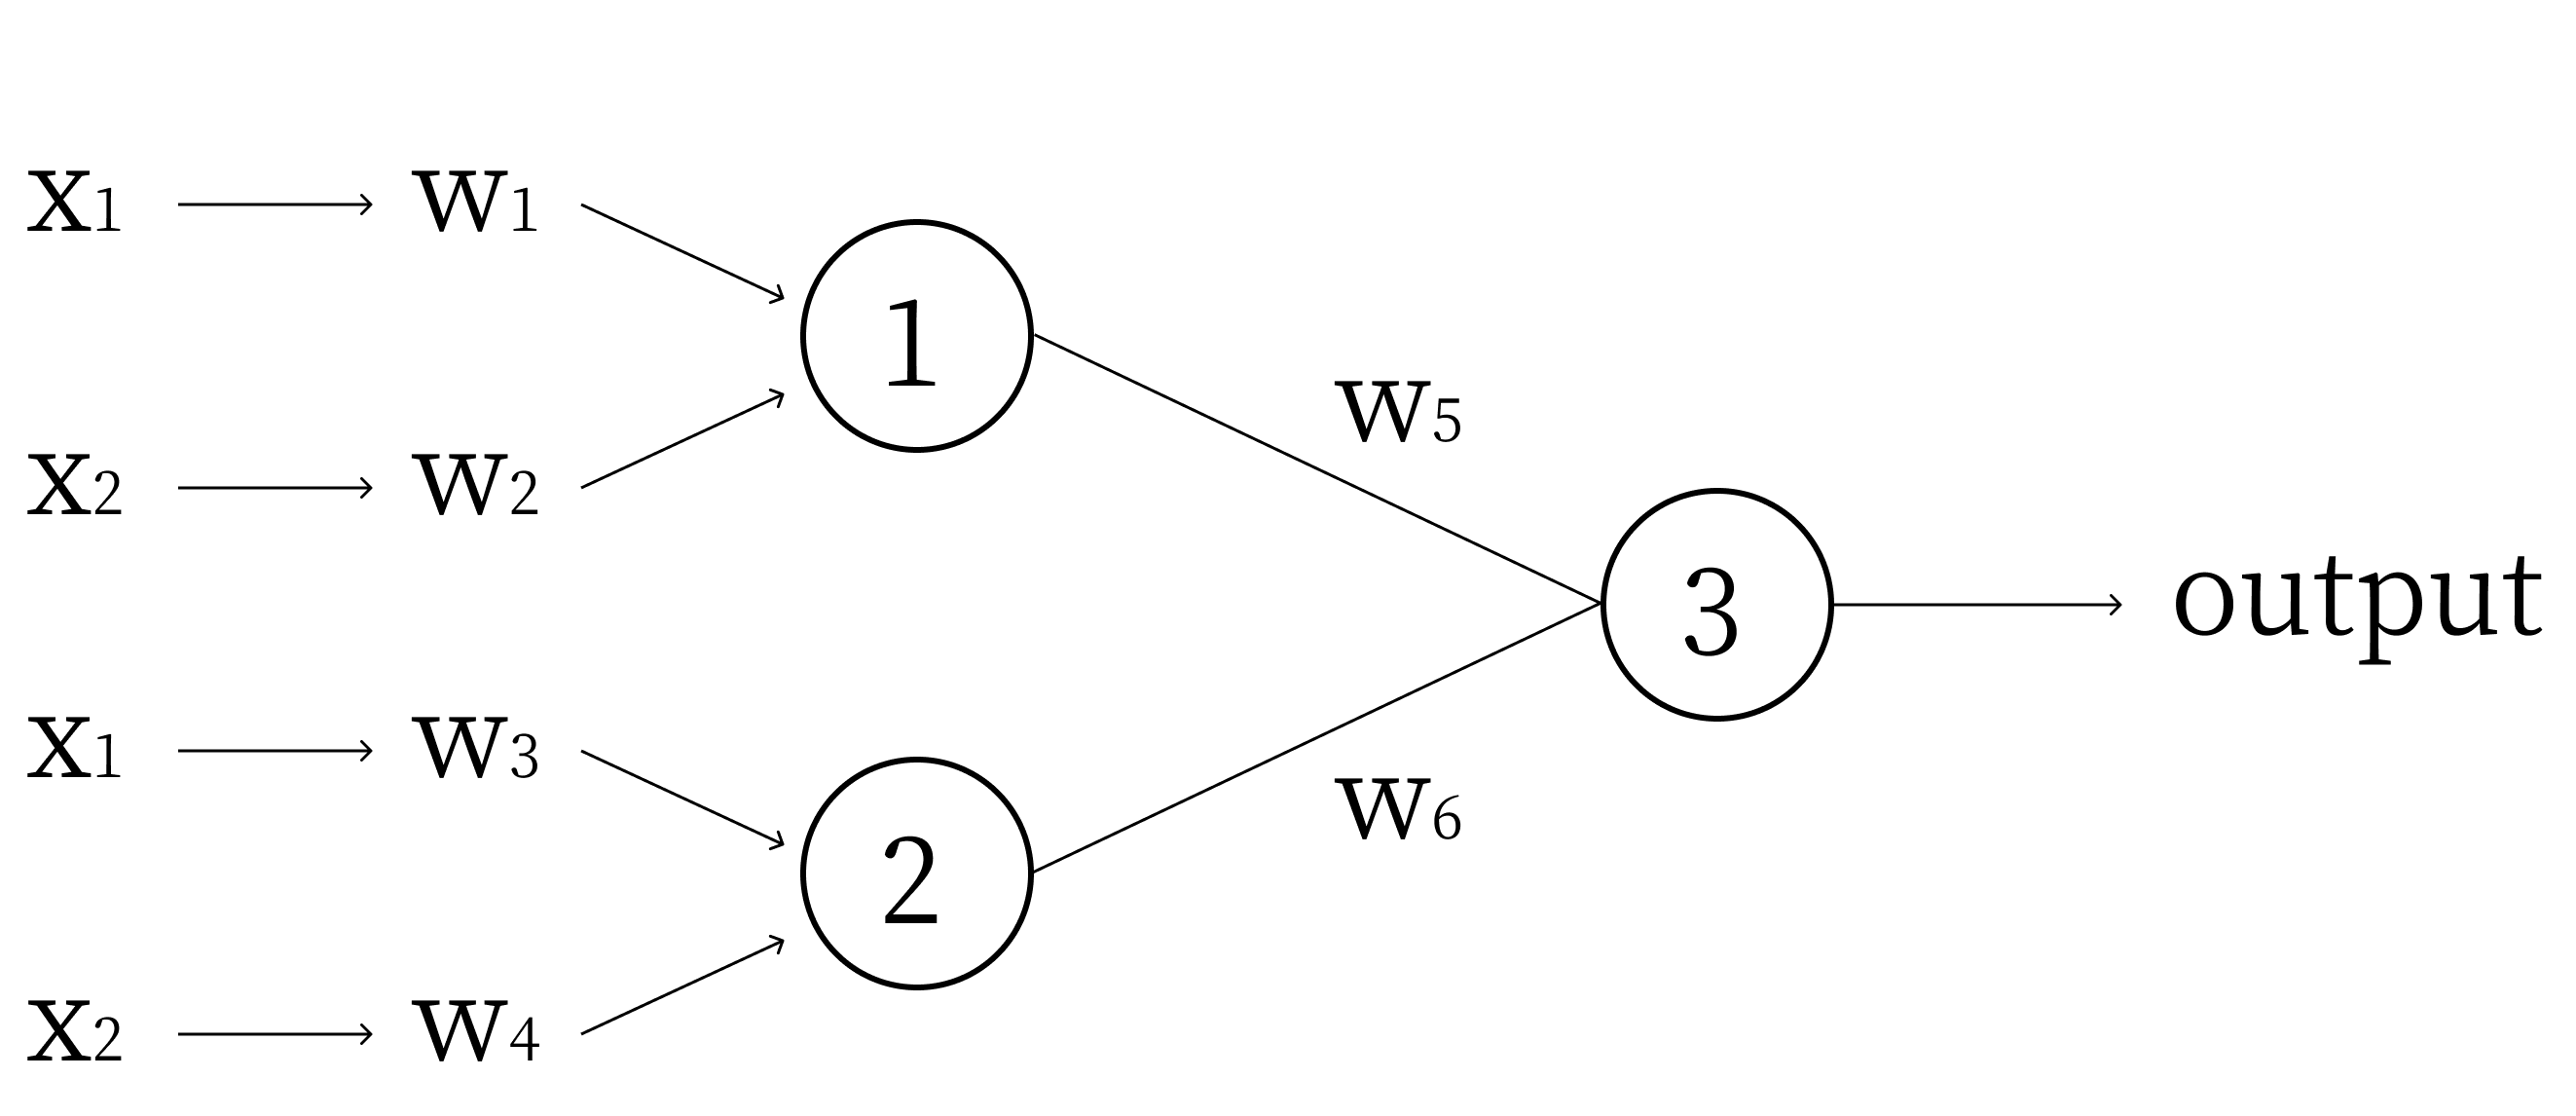
\includegraphics[scale=0.3]{Frame}
\end{center}

Let perceptron 1 model $y + x - 1.5 = 0$ (the upper line), and perceptron 2 model $y + x - 0.5 = 0$ (the lower line). Because the weights are the coefficients of these functions, $w_1 = 1, w_2 = 1, w_3 = 1, w_4 = 1$ and the biases $b_1 = -1.5$ and $b_2 = -0.5$.

The output of Perceptron 1 will be a 1 for points above the upper line, and a 0 for the points below the upper line. The output of Perceptron 2 will be a 1 for points above the lower line, and a 0 for points below the lower line. In between the lines, these cancel! However, in order to create a threshold to separate the points between the lines from the points outside, we would like the outputs for points between the lines to be additive.

In other words, we would like the inputs of Perceptron 3 to both be 1 between the lines, and have a maximum of a single 1 for points outside the lines. Thus, we let $w_6 = 1$ and $w_5 = -1$. This gives us an output of $2$ for points between the lines, and a maximum output of 1 for points outside the lines. Thus, we can set the bias for Perceptron 3: $b_3 = -1.5$.

\section{Problems}
\begin{enumerate}
    \item Write out the weights, biases, and structure of the Perceptron that classifies the function OR.
    \item Write out the weights, biases, and structure of the Multi-Layer perceptron that classifies the function XNOR.
    \item Write an implementation of the XOR Multi-Layer Perceptron in Python.
\end{enumerate}


\end{document}
